\documentclass[11pt,a4paper]{article}
\usepackage{epsfig}
\usepackage{amssymb}
\usepackage{latexsym}
%\usepackage{epic}
%\usepackage{eepic}
\usepackage{amsmath}
\usepackage{verbatim}

\textwidth 146 mm
\textheight 230 mm
\oddsidemargin 7mm \evensidemargin -1mm \topmargin -4mm

\author{Jonatan Kallus (kallus@student.chalmers.se)\\
Joel Wilsson (wjoel@student.chalmers.se)}
\date{\today}

\title{Modelling traffic flow}

\begin{document}
\maketitle

\section{Introduction}
Traffic flow can be modelled at a macroscopic level, where traffic flow is
described as a fluid, or at the microscropic level, where the behaviour of
individual cars is described. When modelling traffic as a fluid, there has
to be quite a lot of cars and the gaps in between them must be small. Only
then is it possible to get a reasonable approximation by viewing the traffic
as a continuum. \cite{gazis}

In this project we use a microscopic model, and by stochastic simulations
we gather data about the global characteristics of the system. The model is agent based, a behaviour is defined for individual cars. The interaction of agents creates a system that can be examined.

\section{Model}
The model consists of a \textit{city} and cars of two different types. In this model the city is a non-complete lattice of roads with intersections. All roads have two lanes, one in each direction. The two types of cars differ only in the way their direction is chosen. One type of cars have an assigned goal and uses a path finding algorithm to approach that goal. The other type of car choses a random direction each time it encounters an intersection.

\subsection{Avoiding collisions}
In order to avoid collisions we have implemented locks for all intersections.
A car is not allowed to enter a path which has been locked by another car,
and a car that is about to enter an intersection must lock both the path that
it is going to travel on and all paths crossing that path. If it fails to
lock all paths, it stops and releases the locks currently held. This is a
simplification in our model, but it seems to work well. Intuitively, our
drivers can be thought of as being very careful in intersections.

More complicated strategies to avoid collisions are possible and, in some
cases, more realistic. For example, if one car enters an intersection and
a car following it is going in the same direction, both cars can be in
the same intersection at the same time without colliding. This kind of
behaviour is not possible with our solution. Such complicated behaviour
would be difficult to implement properly, but such ``stop and yield''
intersections are supported in more advanced traffic simulation
software such as CORSIM. \cite{comparison}

\subsection{Generating a random city}
A random city is generated by taking a two dimensional lattice with a certain \textit{width} and \textit{height}. The lattice is fully connected initially, with a four-way intersection at each node in the lattice. As a second step connections are removed in the lattice until a certain fraction of the original edges remains. This fraction parameter will be called \textit{connectivity}. This removal of edges causes some of the four-way intersections to become three-way intersections, turns or ordinary straight roads.

The city is created in this way to be more realistic and to show more interesting characteristics possibly causing some road parts to be used more often and others to be used less often.

In summary, the generation of the city for the model contributes with three parameters for the model: width, height and connectivity.
\subsection{Car types}
As mentioned earlier, the model has two types of cars, random cars and cars with goals. The two types are choosen to make the model as simple as possible, but to still show some interesting and measurable behavior.

Cars of both types have their traffic behaviour in common, except for the way their directions are chosen at intersections. All cars have an individual random target velocity from a normal distribution with a \textit{mean velocity} and \textit{velocity deviation}. All cars have the same \textit{target acceleration} for reaching their target velocity and for braking to avoid collitions. All cars have the same \textit{target distance} which they try to keep from cars in front of them. Details of the cars traffic behaviour will be discussed in a later section.
\subsubsection{Random cars}
Random cars are used in the model to add noise and to make cars occur in all parts of the city. The number of random cars will be constant over time, random cars are not created after the initialization of the model and they do not leave the city. The \textit{number of random cars} is an input parameter to the model. As a parallel to reality the random cars can be thought of as taxi cars or residents of the city running local errands. The use of random cars is a simplifications, in reality this behaviour is of course not random.
\subsubsection{Cars with goals}
Cars with goals are introduced at the four corners of the city, and assigned with a randomly chosen other corner at which they will leave the city. The purpose of this car type is to have a way to estimate the effectivity of the traffic network by measuring the time it takes for cars to drive through the city. These cars can be thought of as cars that are not residents of the city but driving through the city with some other city as goal. Cars with goals are entering the city at a constant rate of cars per time unit. The \textit{drive in rate} is an input parameter to the model.
\subsubsection{Path finding}
In order to get a path from the car's current path to the destination we use the
A* path finding algorithm \cite{astar}, which is implemented in the GRAph Theory
for Ruby library (GRATR) \cite{gratr}. In order to be able to use GRATR, a
directed graph is constructed from the map. In this graph, there is a node for
each path in the map and an edge from one node to another if the path
represented by the first node leads to the path represented by the second node.

The A* algorithm does not always find the shortest path, but manual inspection
of the paths chosen for cars showed that it never picked paths that were
unreasonably long. Since we do not require the shortest path, this is
acceptable. Indeed, one could imagine that a driver has some personal reasons
for choosing a slightly longer path, perhaps because he or she enjoys the
scenery of this path.

An alternative would have been to use Dijkstra's path finding algorithm, which
would find the shortest path. This algorithm is also implemented in the GRATR
library, so using it instead of A* is easy. Unfortunately, our graph contains
around 600 nodes and 750 edges, and running Dijkstra's algorithm (as implemented
in GRATR) on this graph takes far too long. We did not consider it worthwhile
to spend time on finding a faster implementation of Dijkstra's path finding
algorithm.

\subsection{Parameters}
In total, the input parameters for the model are width, height and connectivity for the city and mean velocity, velocity deviation, target acceleration, target distance, number of random cars and drive in rate for the cars. The parameters YY will be kept constant at values that produces a basis for interesting and measurable behaviors. ZZ will be varied and their effect on the model will be examined.

\section{ODE description of car velocity}
The most important factor for the acceleration of a car is the relative speed between the leading and
the following car. This leads to the following ordinary differential equation for the acceleration of a car following a leading car \cite{gazis}:
\begin{equation}
\label{ode}
\frac{d^2 x_{n+1}(t + T)}{dt^2} = \lambda \left[ \frac{dx_n(t)}{dt} - \frac{dx_{n+1}(t)}{dt} \right] 
\end{equation}
where n denotes the number corresponding to the lead car, $n+1$ that of the
following car, T is the reaction time lag, and $\lambda$ is a coefficient of
proportionality of the driver reaction to the stimulus. $\lambda$ is known
as the sensitivity coefficient or the gain factor.
In this project we use a constant sensitivity coefficient.

Since there is a time lag, each car keeps a record of its previous speeds
as far back as the time lag requires. A following car can then use this
``speed history'' to solve the ordinary differential equation above to
update their acceleration.

A car which does not have second car in front of it which is sufficiently
close for the first car to be considered as following the second, the first car will not
use equation \ref{ode}. Instead, it will use a constant acceleration.

If we simplify \ref{ode} by letting $\frac{dx_n(t)}{dt}=c$, $c$ constant, and
$T=0$ we get an ODE which is easy to solve analytically.
$$
\frac{d^2 x(t)}{dt^2} = \lambda \left[ c - \frac{dx(t)}{dt} \right] 
$$
Here, we could safely drop the indices on $x$ since the equation now only
involves one car. The equation can be written as a system of first order
equations:
\begin{eqnarray*}
\frac{dx_1}{dt} &=& x_2 \\
\frac{dx_2}{dt} &=& \lambda c - \lambda x_2
\end{eqnarray*}
The second equation can be solved using its integrating factor and thereafter
the first equation is trivial to solve.
\begin{eqnarray*}
&\frac{dx_2}{dt} + \lambda x_2 = \lambda c \\
&e^{t\lambda}\frac{dx_2}{dt}+e^{t\lambda}\lambda x_2 = e^{t\lambda}\lambda c \\
&\frac{d\left(e^{t\lambda}x_2\right)}{dt} = e^{t\lambda}\lambda c \\
&e^{t\lambda}x_2 = e^{t\lambda}c + A \\
&x_2 = c + e^{-t\lambda}A \\
\end{eqnarray*}
\begin{eqnarray*}
&\frac{dx_1}{dt}=x_2 \\
&x_1 = \int x_2 dt + B \\
&x_1 = ct - \frac{e^{-t\lambda}}{\lambda}A + B
\end{eqnarray*}

\begin{figure}[ht]
\centering
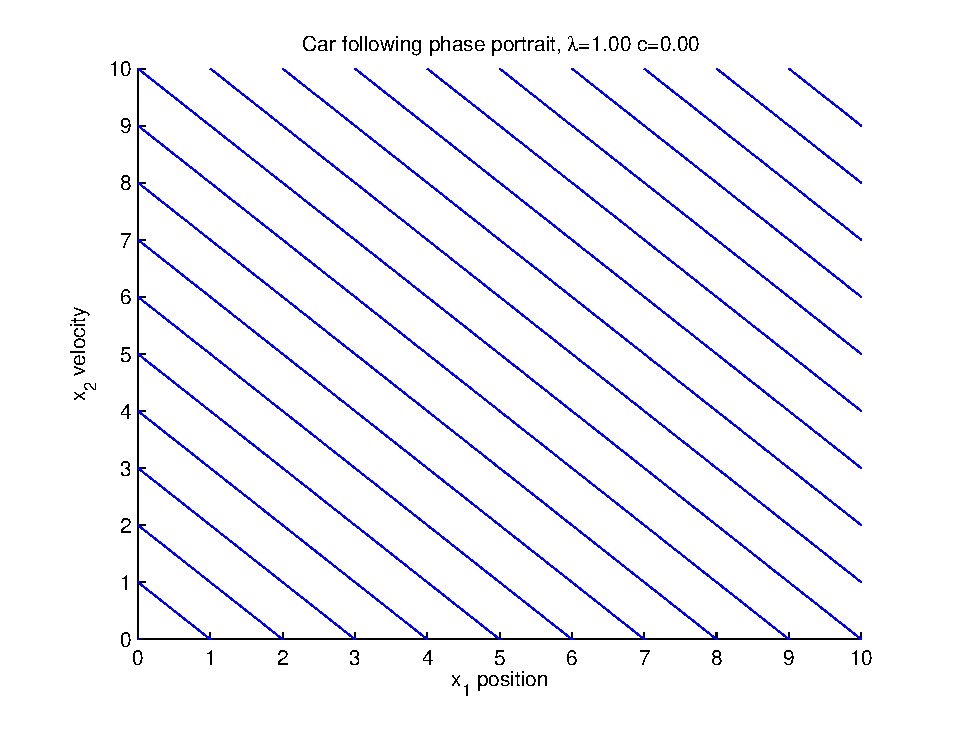
\includegraphics[width=400pt]{phase1-0}
\caption{Phase portrait for simplified ODE.}
\label{phase1-0}
\end{figure}

\begin{figure}[ht]
\centering
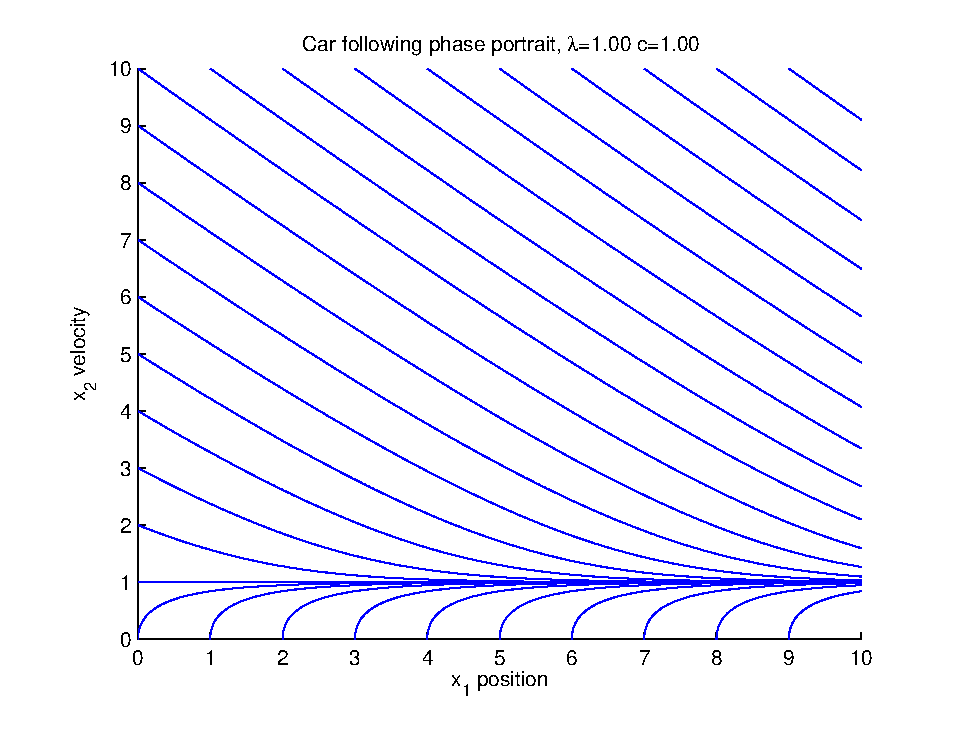
\includegraphics[width=400pt]{phase1-1}
\caption{Phase portrait for simplified ODE.}
\label{phase1-1}
\end{figure}

\begin{figure}[ht]
\centering
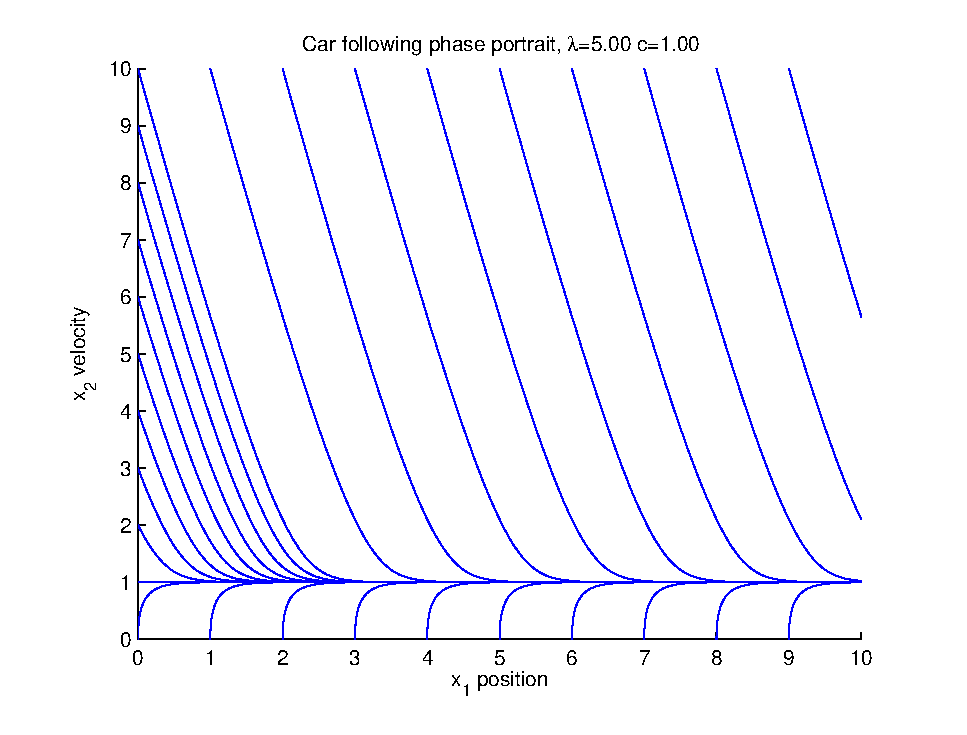
\includegraphics[width=400pt]{phase5-1}
\caption{Phase portrait for simplified ODE.}
\label{phase5-1}
\end{figure}

\begin{figure}[ht]
\centering
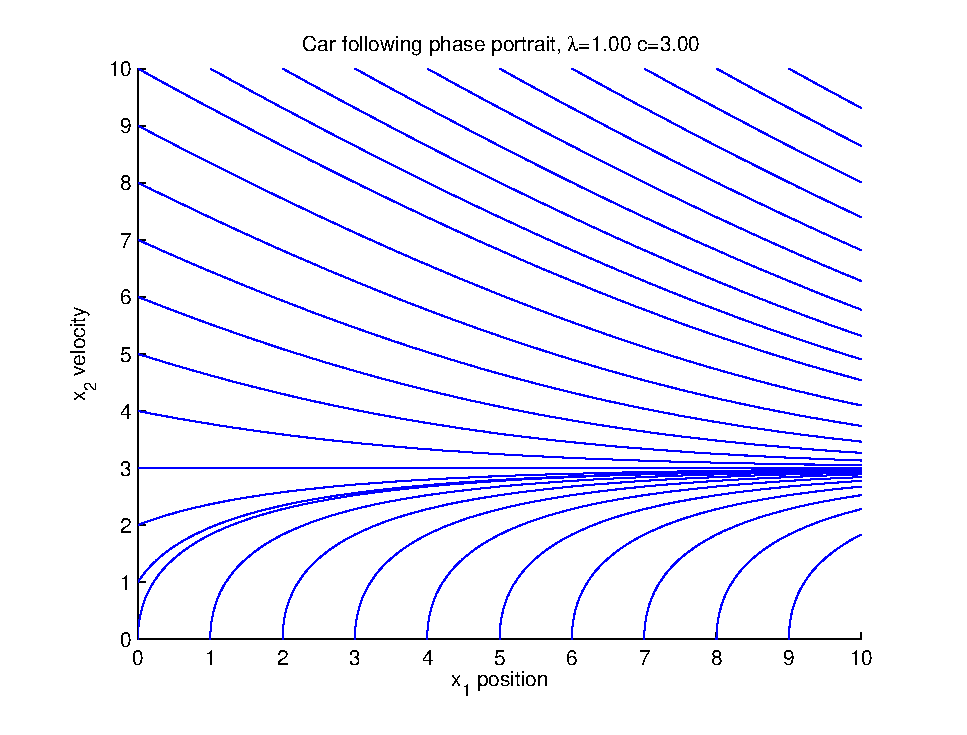
\includegraphics[width=400pt]{phase1-3}
\caption{Phase portrait for simplified ODE.}
\label{phase1-3}
\end{figure}

Phase portraits for the simplified version of equation \ref{ode} were constructed and are
presented in figures \ref{phase1-0}, \ref{phase1-1}, \ref{phase5-1} and
\ref{phase1-3}. For
$c=0$, all points on the horizontal line $x_2=0$ are unstable fixed points. For
$c \neq 0$ there are no fixed points. A higher $\lambda$ makes the speed
approach $c$ faster. As can be seen when comparing figures \ref{phase1-1} and
\ref{phase1-3}, cars aproach a lower speed faster than a higher speed.

\begin{figure}[ht]
\centering
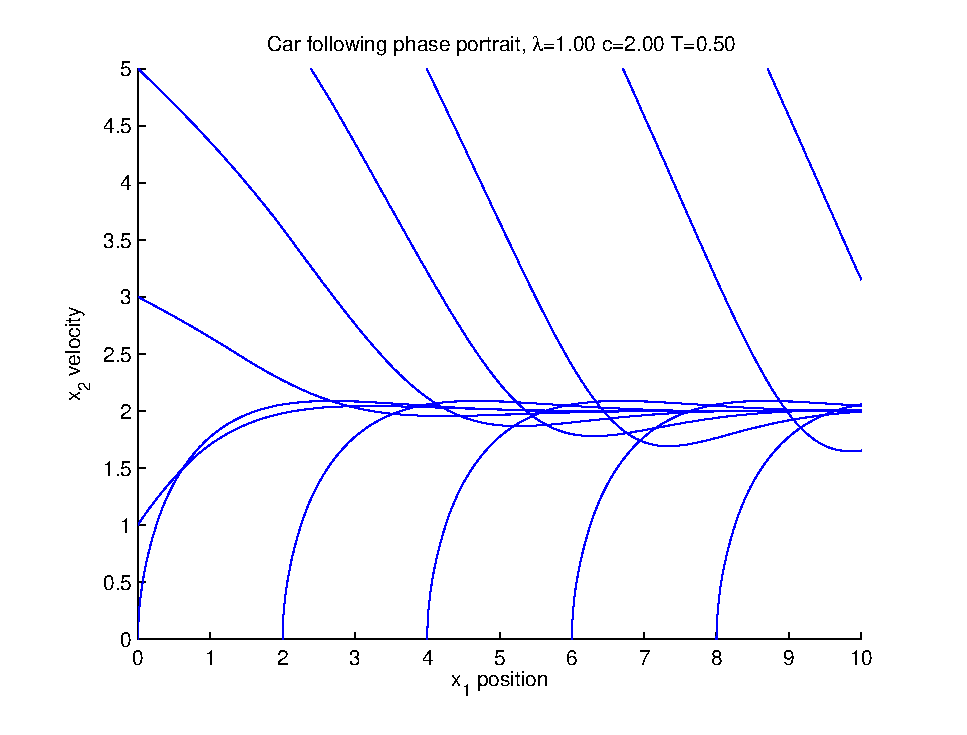
\includegraphics[width=400pt]{phasedelay1-2-05}
\caption{Phase portrait for ODE, numerically computed.}
\label{phasedelay1-2-05}
\end{figure}

\begin{figure}[ht]
\centering
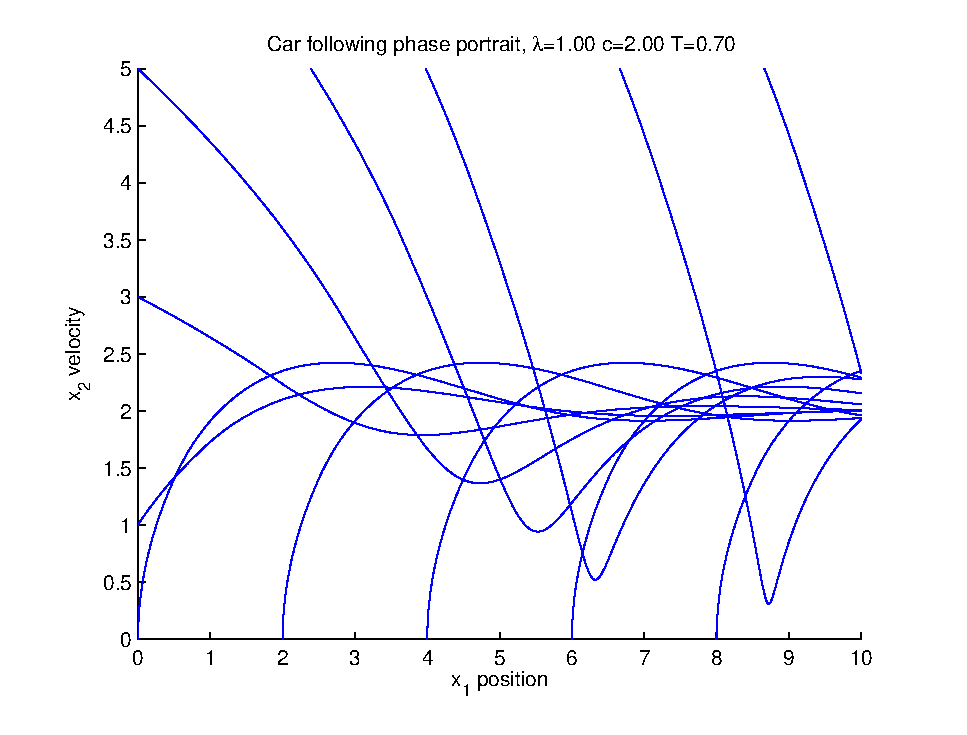
\includegraphics[width=400pt]{phasedelay1-2-07}
\caption{Phase portrait for ODE, numerically computed.}
\label{phasedelay1-2-07}
\end{figure}

It is possible to make a numerical investigation of the ODE with a time delay.
Equation \ref{ode} can be written as a system of first order equation
\begin{eqnarray*}
\frac{dx_1(t)}{dt} &=& x_2(t) \\
\frac{dx_2(t)}{dt} &=& \lambda \left( c - x_2(t-T) \right)
\end{eqnarray*}
with the discrete counterpart
\begin{eqnarray*}
\Delta x_1 &=& \Delta t x_2 \\
\Delta x_2 &=& \lambda \Delta t ( c - x_{2,T})
\end{eqnarray*}
where $x_{2,T}$ is the value of $x_2$ approximately $T$ time units back.

The trajectories were calculated numerically, and are presented in figures
\ref{phasedelay1-2-05} and \ref{phasedelay1-2-07}. We can see how the speed of
the car overshoots the target speed because of the time delay. MATLAB code for
the numerical computation is presented last in this paper. When letting $T=0$
the phase portraits are identical to the analytical solution of the simplified
ODE, which validates our calculations.

\subsection{Gap acceptance}
In the real world, a driver sitting in a queue usually does not start moving his car as
soon as the car in front starts to move. Instead, he waits until there are a few meters
between the cars before he considers it worth driving forwards a small distance.
This is modelled using a gap acceptance function $\alpha(G)$:
\[ \alpha(G) = 0, G < T\\
\alpha(G) = 1 - \exp{-\lambda(G - T)} \]
where $G$ is the gap distance and $T$ is the minimum gap that will be accepted.
$\alpha(G)$ is the \emph{probability} that the driver will move when there is a gap $G$
to the next car. We use a minimum gap set to the length of one car in our simulation.

To prevent cars from stopping unreasonably far from a stopped target (either a car or a
locked crossing), a small term \[ \delta (D - W) \] is added to the acceleration,
where $D$ is the distance to the next obstacle and $W$ is the wanted distance to the next target.
Our simulation is using $\delta = 0.005$ and $W$ set to half of the length of a car.

\subsection{Stability}
\subsection{Phase portrait}

\section{Fundamental characteristics of road traffic}
\subsection{The fundamental diagram of road traffic}

%\section{Modelling traffic flow as a fluid}

\section{How parameters affect throughput}

\section{MATLAB code}
\subsection{Plot of analytical solution of simplified ODE}
\begin{verbatim}
t = linspace(0,10,1000);
c = 3;
lambda = 1;
figure(1);
clf;
axis([0 10 0 10]);
hold on;
xlabel('x_1 position');
ylabel('x_2 velocity');
title(sprintf('Car following phase portrait,
  \\lambda=%.2f c=%.2f',lambda,c));
starts = [0 10; 1 10; 2 10; 3 10; 4 10; 5 10;...
    6 10; 7 10; 8 10; 9 10;...
    0 0; 1 0; 2 0; 3 0; 4 0; 5 0; 6 0; 7 0;...
    8 0; 9 0;...
    0 1; 0 2; 0 3; 0 4; 0 5; 0 6; 0 7; 0 8; 0 9];
for i = 1:29
    x1_0 = starts(i,1);
    x2_0 = starts(i,2);
    B = x2_0 - c;
    A = x1_0 + B/lambda;
    x1 = c*t - exp(-lambda*t)*B/lambda + A;
    x2 = c + exp(-lambda*t)*B;
    plot(x1,x2);
end

\end{verbatim}

\subsection{Numerical computation of phase portrait for ODE with delay}
\begin{verbatim}
c = 2;
lambda = 1;
T = 0.5;

figure(1);
clf;
axis([0 10 0 5]);
hold on;
xlabel('x_1 position');
ylabel('x_2 velocity');
title(sprintf('Car following phase portrait,
  \\lambda=%.2f c=%.2f T=%.2f',lambda,c,T));

starts = [2 10; 4 10; 6 10; 8 10;...
    0 0; 2 0; 4 0; 6 0; 8 0;...
    0 1; 0 3; 0 5; 0 7; 0 9];

for i = 1:29
    ts = linspace(0,10,1000);
    dt = diff(ts); dt = dt(1);
    x1 = starts(i,1);
    x2 = starts(i,2);
    x1s = [x1];
    x2s = [x2];
    for t = ts
        old_x2 = x2s(end-min(round(T/dt), numel(x2s)-1));
        x2 = x2 + lambda * dt * (c - old_x2);
        x1 = x1 + dt * x2;
        x1s = [x1s x1];
        x2s = [x2s x2];
    end
    plot(x1s, x2s);
end
\end{verbatim}

\begin{thebibliography}{99}
\bibitem{haight} Frank A. Haight
{\it Mathematical theories of traffic flow} {\bf 1963}

\bibitem{gazis} Denos C. Gazis
{\it Traffic Theory} {\bf 2002}

\bibitem{gratr} Shawn Patrick Garbett
{\it GRAph Theory in Ruby (GRATR)} {\bf 2006}

\bibitem{astar} P. E. Hart, N. J. Nilsson, B. Raphael
{\it A Formal Basis for the Heuristic Determination of Minimum Cost Paths} {\bf 1968}

\bibitem{comparison} Steven L. Jones, Jr, et al
{\it TRAFFIC SIMULATION SOFTWARE COMPARISON STUDY} {\bf 2004}
%\bibitem{wiki} Wikipedia
%{\it Entry for the Ising model} {\bf 2011}

\end{thebibliography}

\end{document}
